\chapter{Experiments and Results}


\section{Introduction}

In chapter 2 we saw that the problem is to determine the image(i.e intensity distribution) from an incomplete set of Fourier measurements since we have data available only at certain points in the Fourier domain, determined by the $u-v$ coverage of the antenna setup. The performance of our reconstruction algorithm depends both on the intensity distribution that we wish to recover and the {\emph sampling map}. Here, sampling map refers to the points in the Fourier domain where data is available. Such points are referred to as {\emph sampled points} or {\emph sampling points}. In practice this depends on the $u-v$ coverage of the antenna setup where both $u$ and $v$ can take any real value. In order for the Fourier relationship to be valid while using fast Fourier transforms, the $u-v$ plane must correspond to a set of $m \times n$ uniformly spaced frequencies. This is achieved by the process of gridding as discussed in \cite{GMRT}. .
We will consider experiments where we wish to recover two images simultaneously and where we assume that the information overlap is known. Note that this in general will require registration but in this work we will assume that registration has been done and concentrate on getting better reconstructions based on the information overlap between the two images. We will refer to the two images as the ``left'' and ``right'' images or simply as image ``$x$'' and image ``$y$''. We conduct three class of experiments on simulated data:
\begin{enumerate}
 \item Experiments on images consisting of astronomical point sources that are sparse in spatial domain.
 \item Experiments on the Shepp-Logan phantom, a representative image that is compressible in wavelet domain and used in MRI applications.
  \item Experiments on images consisting of both astronomical point and extended sources.
\end{enumerate}

\section{Experiments on point sources}
\begin{enumerate}
\item Here we consider images consisting of point sources such as clusters of stars.
\item We consider the problem in Formulation-3 where the objective function that we wish to minimize is as in Eq. {eq:formu} repeated here for convenience:
 \begin{equation}
 F(z_x, z_y) = \|\Phi_x\Psi z_x - b_x\|_2^2 + \|\Phi_y\Psi z_y - b_y\|_2^2 + \lambda_x \|z_x\|_1 + \lambda_y \|z_y\|_1 + \mu || B_x z_x - B_y z_y||_2^2.
 \end{equation}
 Also since,
\begin{eqnarray}
	x &=& \Psi z_x 	\label{eq:domainx}\\
	y &=& \Psi z_y,
	\label{eq:domainy}
\end{eqnarray}
and our images are sparse in spatial domain itself we have $\Psi = I$, the identity matrix.
\item We will assume that there is an overlap of $S$ pixels between the two reconstructed images and $B_x$ and $B_y$ represent the matrices that extract the portions that will overlap in matching order.
\item Since our image sizes are typical $256 \times 256$, it is infeasible to store the matrices $\Phi_x, \Phi_y,  B_x $ and $B_y$ and perform actual matrix multiplication due to their huge sizes. Instead we use them as operators.
\item $\Phi_x$ and $\Phi_y$ are implemented using the Fast Fourier transform operator. $B_x$ and $B_y$ just represent selecting certain portions of the image and rearranging them in correct order which can also be done without any matrix multiplication.
\item The alternating algorithm requires us to also use the transpose of the above matrices and thus we also represent $\Phi_x^T, \Phi_y^T, B_x^T$ and $B_y^T$ by operators.
\item The Lipschitz constants $L_x$ and $L_y$ are determined by differentiating the function the smooth part of the function $F(z_x, z_y)$ and applying the definition of the Lispchitz constant in Eq. \ref{eq:lip}:
\begin{eqnarray}
L_x &=& 2\max(eig( \Phi_x^T \Phi_x))  +  2 \mu \max(eig( B_x^T B_x)) \\
L_y &=& 2\max(eig( \Phi_y^T \Phi_y))  +  2\mu \max(eig( B_y^T B_y))
\end{eqnarray}This value can be upper bounded by $2(1 + \mu)$, where $\mu$ is the weight to the coupling term.
\item The error measure $e$, we use in all our experiments is the relative error and is given by
\begin{equation}
	e = \frac{\|x_r - x\|_F}{\|x \|_F},
\end{equation}
where $x_r$ refers to the reconstructed image and $x$ refers to the original image and $\| \|_F$ refers to the Frobenius norm.

\end{enumerate}
 We conducted two experiments using the ISTA based alternating algorithm as follows:
\subsubsection{Experiment with 33\% overlap}
\begin{enumerate}
\item The two $256 \times 256$ images consist of 175 stars each with an overlap between the last 85 columns of the left image with the first 85 columns of the right image. The stars of size 1 pixel each and have intensity value 1. The star locations are chosen uniformly at random.
\vspace{-0.2in}

\begin{figure}[H]

%\begin{center}  \vspace{-0.1in}
	\hspace{-0.5in}
\subfigure[Left image]{
	\includegraphics[width=4in]{images/expt1/1a.png}
		}
		\hspace{-1in}
\subfigure[Right image]{
	\includegraphics[width=4in]{images/expt1/1b.png}
		}
\caption [Original images, 175 stars, 33 \% overlap]{Original left and right images, 175 stars. The last 85 columns of the left image overlap with the first 85 columns of the right image.}
\label{fig:expt11}
%\end{center}
\end{figure}
 \begin{figure}[H]
	\centering \vspace{-0.1in}
	\includegraphics[width=2.5in]{images/expt1/2.png}
	 \caption[GMRT sampling map for an instant ]{\small GMRT sampling map for an instant. The white pixels correspond to locations where fourier data is available}
	\label{fig:expt12}
\end{figure}

\item The star locations are picked uniform randomly and the intensity of each star is chosen uniformly between $[0.3, 1]$. The two color coded original images are shown in Fig. \ref{fig:expt11} with the background sky as black and color of stars varying from blue to red as intensity increases.


\item For both left and right images, Fourier measurements are available as per the GMRT sampling map for an instant consisting of 746 points as shown in Fig. \ref{fig:expt12}.  Thus $\Phi_x = \Phi_y$.

\begin{figure}[t!]
\hspace{-0.5in}
%\begin{center}  \vspace{-0.1in}
\subfigure[Left image]{
	\includegraphics[width=4in]{images/expt1/3a.png}
		}
		\hspace{-1in}
\subfigure[Right image]{
	\includegraphics[width=4in]{images/expt1/3b.png}
		}
\caption [Dirty images, 175 stars, 33\% overlap, 746 points,  rms $1e^{-4}$]{Dirty images, 175 stars, 33\% overlap, 746 points, rms $1e^{-4}$}
\label{fig:expt13}
%\end{center}
\end{figure}


\item We consider additive white gaussian noise with a rms value of $1e^{-4}$.
\item For the initial guesses for $z_x$ and $z_y$ we first find the dirty images by performing a direct Fourier inverse while setting zeros at locations where Fourier data is not available. We then extract the corresponding $z_x$ and $z_y$ which in this case are the images themselves since $\Psi = I$ and use these as starting points. The dirty images are shown in Fig. \ref{fig:expt13}.

\item We choose $\mu = 0$ and $\mu = 0.01$ where in the first case there is no coupling and in the second case coupling is present. We use $\lambda_x = \lambda_y = \lambda$ and vary it in the logarithmic scale between [-3.75, -2.75] in steps of size 0.25. 
\item We terminate the algorithm either when the relative difference in value of objective function is less than $1e^{-7}$ or when we reach 30000 iterations.
\item The relative error vs.  $\lambda$ graphs for the left and right images are shown in Fig. \ref{fig:expt14}.

\vspace{-0.2in}
\begin{figure}[H]

%\begin{center}  \vspace{-0.1in}
\subfigure[Left image]{
	\includegraphics[width=3in]{images/expt1/4a.png}
		}
\hspace{-0.1in}
\subfigure[Right image]{
	\includegraphics[width=3in]{images/expt1/4b.png}
		}
\caption [Error vs $\lambda$, 175 stars, 33\% overlap, 746 points,  rms $1e^{-4}$]{Error vs $\lambda$, 175 stars, 33\% overlap, 746 points, rms $1e^{-4}$}
\label{fig:expt14}
%\end{center}
\end{figure}

\item The reconstructed left and right images for $\lambda = 1e^{-3.25}$ for the two values of $\mu$ are shown in Fig. \ref{fig:expt15} and  Fig. \ref{fig:expt16} respectively. The comparison of the zoomed regions highlighted by the boxes are with corresponding regions from the original images are shown in Fig. \ref{fig:expt17}  and Fig. \ref{fig:expt18}.


\vspace{-0.2in}
\begin{figure}[H]
\hspace{-0.5in}
%\begin{center}  \vspace{-0.1in}
\subfigure[Coupled($\mu = 0.01$) ]{
	\includegraphics[width=4in]{images/expt1/5a.png}
		}
\hspace{-1in}
\subfigure[Separate($\mu = 0$)]{
	\includegraphics[width=4in]{images/expt1/5b.png}
		}		
\caption [Reconstructed left images, 175 stars, 33\% overlap, 746 points,  rms $1e^{-4}$, $\lambda = 1e^{-3.25}$]{Reconstructed left images, 175 stars, 33\% overlap, 746 points, rms $1e^{-4}$, $\lambda = 1e^{-3.25}$}
\label{fig:expt15}
%\end{center}
\end{figure}
\vspace{-0.2in}
\begin{figure}[H]
%\begin{center}  \vspace{-0.1in}
\subfigure[Coupled$(\mu = 0.01)$]{
	\includegraphics[width=2.1in]{images/expt1/7a.png}
		}
\hspace{-0.15in}
\subfigure[Separate$(\mu = 0$)]{
	\includegraphics[width=1.9in]{images/expt1/7b.png}
		}
		\hspace{-0.15in}
\subfigure[Original]{
	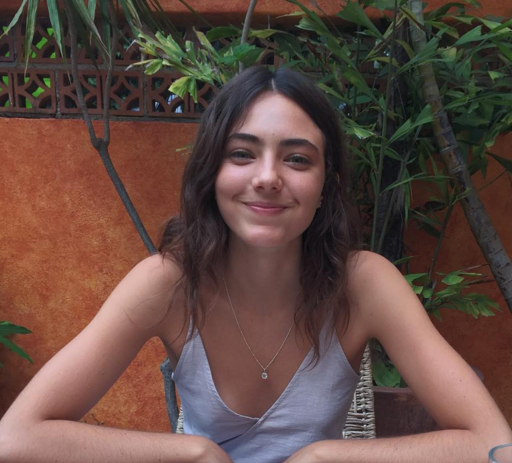
\includegraphics[width=2in]{images/expt1/7c.png}
		}	
\caption [Zoomed left image regions, 175 stars, 33\% overlap, 746 points,  rms $1e^{-4}$, $\lambda = 1e^{-3.25}$]{Zoomed left image regions, 175 stars, 33\% overlap, 746 points, rms $1e^{-4}$, $\lambda = 1e^{-3.25}$ The image using separate formulation has extra blue star near the central red star.}
\label{fig:expt17}
%\end{center}
\end{figure}

\end{enumerate}


\vspace{-0.2in}
\begin{figure}[h!]
\hspace{-0.5in}
%\begin{center}  \vspace{-0.1in}
\subfigure[Coupled($\mu = 0.01$)]{
	\includegraphics[width=4in]{images/expt1/6a.png}
		}
\hspace{-1in}
\subfigure[Separate($\mu = 0$)]{
	\includegraphics[width=4in]{images/expt1/6b.png}
		}		
\caption [Reconstructed right images, 175 stars, 33\% overlap, 746 points,  rms $1e^{-4}$, $\lambda = 1e^{-3.25}$]{Reconstructed right images, 175 stars, 33\% overlap, 746 points, rms $1e^{-4}$, $\lambda = 1e^{-3.25}$}
\label{fig:expt16}
%\end{center}
\end{figure}
\vspace{-0.2in}
\begin{figure}[h!]
%\begin{center}  \vspace{-0.1in}
\subfigure[Coupled$(\mu = 0.01)$]{
	\includegraphics[width=2in]{images/expt1/8a.png}
		}
\hspace{-0.18in}
\subfigure[Separate$(\mu = 0$)]{
	\includegraphics[width=2.1in]{images/expt1/8b.png}
		}
		\hspace{-0.18in}
\subfigure[Original]{
	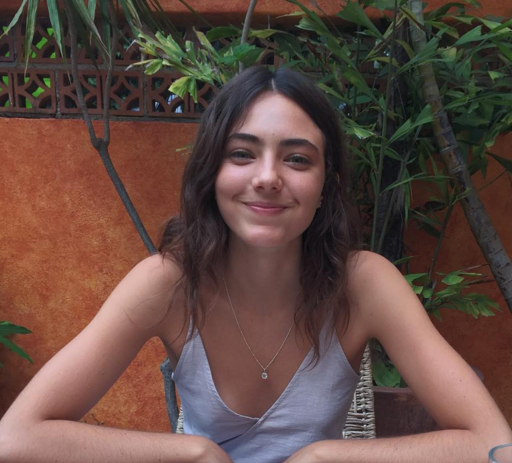
\includegraphics[width=2in]{images/expt1/8c.png}
		}	
\caption [Zoomed right image regions, 175 stars, 33\% overlap, 746 points,  rms $1e^{-4}$, $\lambda = 1e^{-3.25}$]{Zoomed right image regions, 175 stars, 33\% overlap, 746 points, rms $1e^{-4}$, $\lambda = 1e^{-3.25}$.  The image using separate formulation has several excess stars.}
\label{fig:expt18}
%\end{center}
\end{figure}

\subsubsection{Observations}
\begin{enumerate}

\item From Fig. \ref{fig:expt14} we see that the coupled formulation using the alternating algorithm performs better than than the uncoupled formulation. 
\item From Fig. \ref{fig:expt17} and Fig. \ref{fig:expt18} we can see that the reconstructed image in the uncoupled case has both excess stars and missing stars and the coupled formulation not only improves reconstruction in portion of image where overlap occurs but also in regions where there is no overlap.
\item Note that we have a chosen value of $\mu = 0.01$ heuristically since we want to give less weightage to the overlap term as compared to the data fitting terms. 
\item For the best value of $\lambda$ for the left image the error improves from approximately 0.26 to 0.14 and for the right image the error improves from approximately 0.20 to 0.125.
\item Since the level of sparsity in both images and the sampling points are the same in both images both the error and the improvement in error is similar in left and right images.
\end{enumerate}

\subsubsection{Experiment with 50\% overlap}
\begin{enumerate}
\item We repeat the above experiment with same settings except that this time we consider a overlap of 50\%.
\item The new original images are shown in Fig. \ref{fig:expt21}.

\begin{figure}[t!]
\hspace{-0.5in}
%\begin{center}  \vspace{-0.1in}
\subfigure[Left image]{
	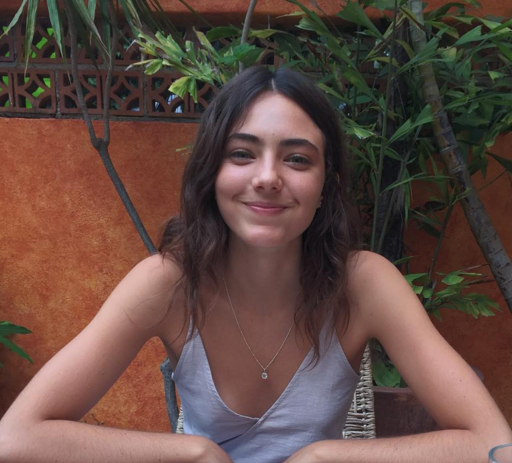
\includegraphics[width=4in]{images/expt1/9a.png}
		}
		\hspace{-1in}
\subfigure[Right image]{
	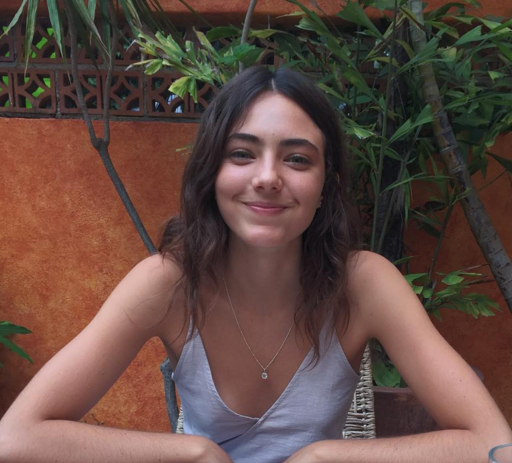
\includegraphics[width=4in]{images/expt1/9b.png}
		}
\caption [Original images, 175 stars, 50\% overlap]{Original left and right images, 175 stars. The last 85 columns of the left image overlap with the first 128 columns of the right image.}
\label{fig:expt21}
%\end{center}
\end{figure}
\item The sampling map, noise rms value, the values of $\mu$ and values of $\lambda$ are same as in the previous experiment.
\item The relative error vs.  $\lambda$ graphs for the left and right images are shown in Fig. \ref{fig:expt22}.

\begin{figure}[b!]

%\begin{center}  \vspace{-0.1in}
\subfigure[Left image]{
	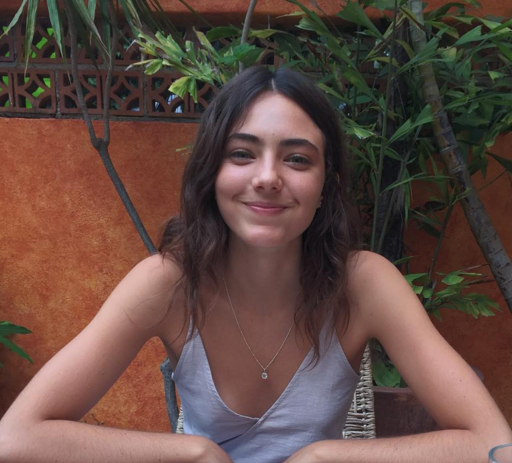
\includegraphics[width=3in]{images/expt1/10a.png}
		}
\hspace{-0.1in}
\subfigure[Right image]{
	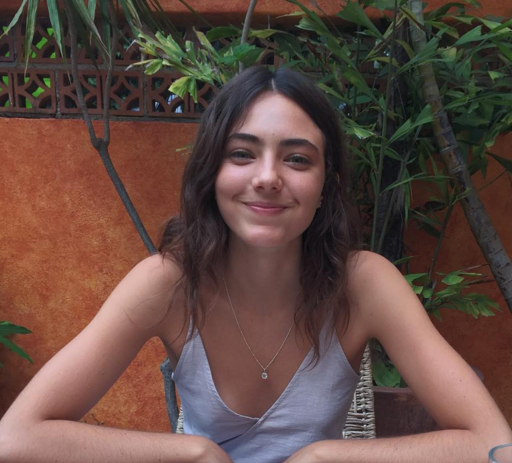
\includegraphics[width=3in]{images/expt1/10b.png}
		}
\caption [Error vs $\lambda$, 175 stars, 50\% overlap, 746 points,  rms $1e^{-4}$]{Error vs $\lambda$, 175 stars, 50\% overlap, 746 points, rms $1e^{-4}$}
\label{fig:expt22}
%\end{center}
\end{figure}

\item The reconstructed left and right images for the best values of $\lambda$ for the two values of $\mu$ are shown in Fig. \ref{fig:expt15} and  Fig. \ref{fig:expt16} respectively. 

\vspace{-0.2in}
\begin{figure}[h!]
\hspace{-0.5in}
%\begin{center}  \vspace{-0.1in}
\subfigure[Coupled, $\mu = 0.01, \lambda = 1e^{-3.5}$]{
	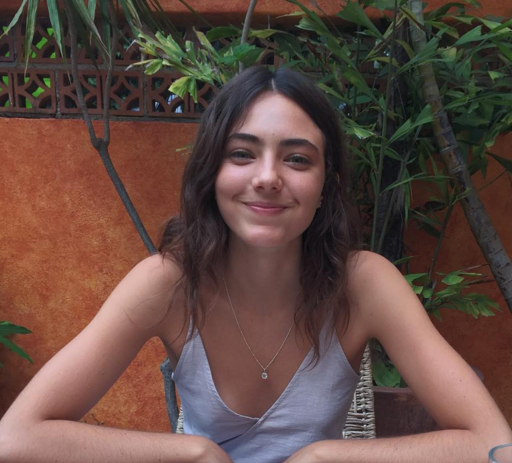
\includegraphics[width=4in]{images/expt1/11a.png}
		}
\hspace{-1in}
\subfigure[Separate, $\mu = 0, \lambda = 1e^{-3.25}$]{
	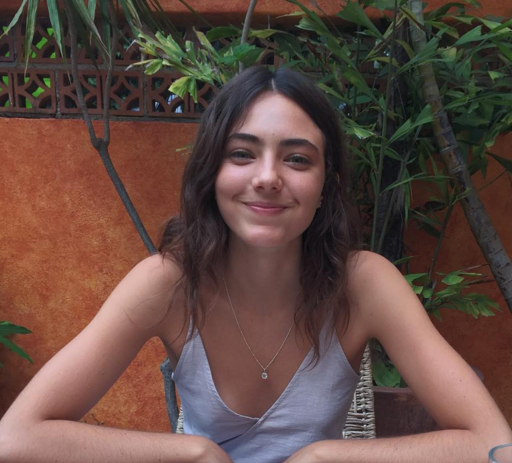
\includegraphics[width=4in]{images/expt1/11b.png}
		}		
\caption [Reconstructed left images, 175 stars, 50\% overlap, 746 points,  rms $1e^{-4}$]{Reconstructed left images, 175 stars, 50\% overlap, 746 points, rms $1e^{-4}$. The image using separate formulation has several excess star in the central region.}
\label{fig:expt15}
%\end{center}
\end{figure}

\begin{figure}[t!]
\hspace{-0.5in}
%\begin{center}  \vspace{-0.1in}
\subfigure[Coupled, $\mu = 0.01, \lambda = 1e^{-3.5}$]{
	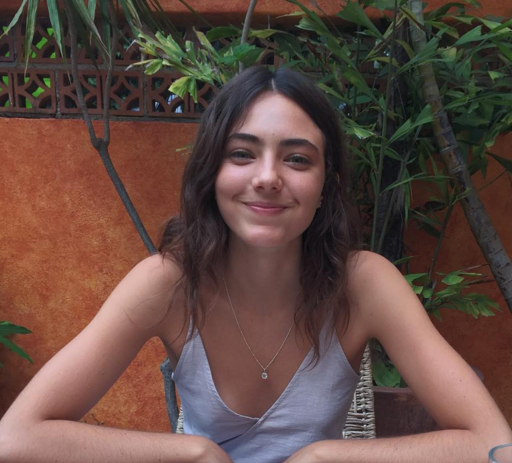
\includegraphics[width=4in]{images/expt1/12a.png}
		}
\hspace{-1in}
\subfigure[Separate, $\mu = 0, \lambda = 1e^{-3.25}$]{
	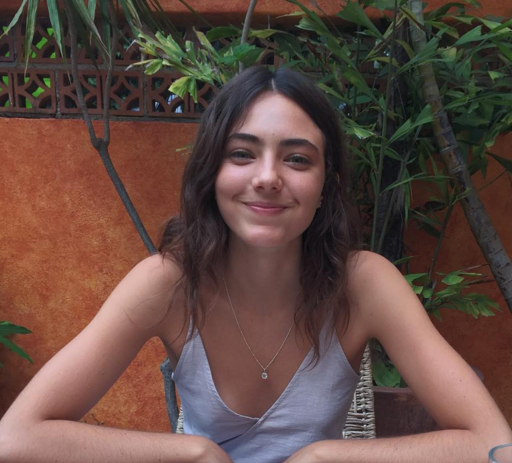
\includegraphics[width=4in]{images/expt1/12b.png}
		}		
\caption [Reconstructed right images, 175 stars, 50\% overlap, 746 points,  rms $1e^{-4}$]{Reconstructed right images, 175 stars, 50\% overlap, 746 points, rms $1e^{-4}$. The image using separate formulation has several excess star in the central region.}
\label{fig:expt16}
%\end{center}
\end{figure}
\end{enumerate}
\subsubsection{Observations}
\begin{enumerate}

\item From Fig. \ref{fig:expt14} and Fig. \ref{fig:expt22} we see that the coupled formulation using the alternating algorithm performs better than than the uncoupled formulation. Also with 50\% overlap the coupled formulation does better than the case where there is 33\% overlap. This is to be expected since with more overlap we have more information and should do better.
\item For the best value of $\lambda$ for the left image the error improves from approximately 0.26 to 0.09 and for the right image the error improves from approximately 0.18 to 0.08.
\item Since the level of sparisity in both images and the sampling points are the same in both images both the error and the improvement in error is similar in left and right images.
\end{enumerate}


\section{Experiments on Shepp-Logan phantom}
\begin{enumerate}
\item In this section we conducted experiments on the Shepp-Logan phantom image, a representative image that is sparse in wavelet domain.
\item We consider the problem in Formulation-3 where the objective function that we wish to minimize is as follows:
 \begin{equation}
 F(z_x, z_y) = \|\Phi_x\Psi z_x - b_x\|_2^2 + \|\Phi_y\Psi z_y - b_y\|_2^2 + \lambda_x \|z_x\|_1 + \lambda_y \|z_y\|_1 + \mu || B_x z_x - B_y z_y||_2^2.
 \end{equation}
 Also since,
\begin{eqnarray}
	x &=& \Psi z_x 	\label{eq:domainx}\\
	y &=& \Psi z_y,
	\label{eq:domainy}
\end{eqnarray}
and our images are sparse in wavelet domain we have $\Psi$ represent an inverse wavelet transform operator.
\item Thus we will first solve for the sparse set of wavelet coefficients and then obtain the reconstructed images using inverse wavelet transform.
\item Since we deal with image sizes of $256 \times 256$ the maximum number of stages we can use is $\log_2(256) = 8$. Also higher the number of stages we use the better sparse approximation we obtain. Thus, we use a 7 stage 2D-DWT with a Haar wavelet to perform the wavelet transform.  In the original images there are approximately 2500 significant coefficients.
\item We will assume that there is an overlap of $S$ pixels between the two reconstructed images and $B_x$ and $B_y$ represent the matrices that take the wavelet coefficients and apply inverse wavelet transform and then extract the portions that will overlap in matching order.
\item The sampling is done by taking slices/lines in the Fourier domain that have equal angular spacing and pass through dc frequency. Thus we have an incomplete set of Fourier measurements obtained by the sampling matrices $\Phi_x$ and $\Phi_y$. We will consider different number lines for the left and right image and observe the performance of the alternating algorithm in this scenario.
\item The Lipschitz constants $L_x$ and $L_y$ are determined as:
\begin{eqnarray}
L_x &=& 2\max(eig( \Phi_x^T \Phi_x))  +  2 \mu \max(eig( B_x^T B_x)) \\
L_y &=& 2\max(eig( \Phi_y^T \Phi_y))  +  2\mu \max(eig( B_y^T B_y))
\end{eqnarray}This value can be upper bounded by $2(1 + \mu)$.
\item The error measure $e$, we use in all our experiments is the relative error and is given by
\begin{equation}
	e = \frac{\|x_r - x\|_F}{\|x \|_F},
\end{equation}
where $x_r$ refers to the reconstructed image and $x$ refers to the original image and $\| \|_F$ refers to the frobenius norm.
\end{enumerate}
We conducted two experiments using the ISTA based alternating algorithm as follows:

\subsubsection{Experiment with 30 and 20 sampling lines}

\begin{enumerate}
\item The left and right original images of size $256 \times 256$ images  in Fig. \ref{fig:expt31} consist of the Shepp-Logan phantom with an overlap between the last 128 columns of the left image with the first 128 columns of the right image. 
\begin{figure}[b!]

%\begin{center}  \vspace{-0.1in}
\hspace{0.4in}
\subfigure[Left image]{
	\includegraphics[width=2.5in]{images/expt3/1a.png}
		}
		\hspace{0.2in}
\subfigure[Right image]{
	\includegraphics[width=2.5in]{images/expt3/1b.png}
		}
\caption [Original images, Shepp-Logan phantom, 50\% overlap]{Original left and right images, Shepp-Logan phantom. The last 128 columns of the left image overlap with the first 128 columns of the right image.}
\label{fig:expt31}
%\end{center}
\end{figure}

\item Fourier data is available at locations given by the sampling map which consist of 30 lines (10501 points) and 20 lines (6657 points) respectively for the left and right image as shown in Fig. \ref{fig:expt32}
\begin{figure}[!t]
\hspace{-0.5in}
%\begin{center}  \vspace{-0.1in}
\subfigure[Left image]{
	\includegraphics[width=4in]{images/expt3/1c.png}
		}
		\hspace{-1in}
\subfigure[Right image]{
	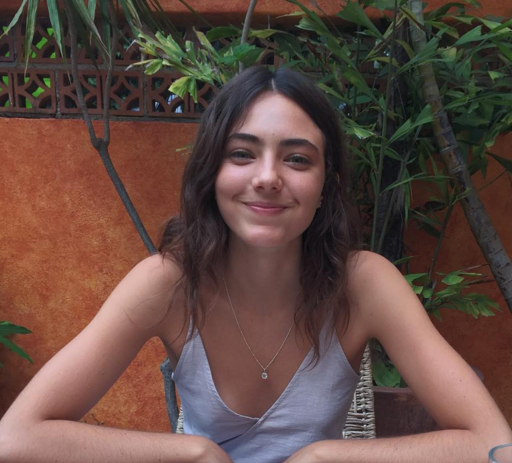
\includegraphics[width=4in]{images/expt3/1d.png}
		}
\caption [Sampling maps, Left 30 lines, Right 20 lines]{Sampling maps, Left 30 lines, Right 20 lines}
\label{fig:expt32}
%\end{center}
\end{figure}

\item We consider additive white gaussian noise with a rms value of $1e^{-4}$.
\item For the initial guesses for $z_x$ and $z_y$ we first find the dirty images by performing a direct Fourier inverse while setting zeros at locations where Fourier data is not available. We then extract the corresponding $z_x$ and $z_y$ which in this case are the wavelet coefficients corresponding to the dirty image and use these as starting points. The dirty images are shown in Fig. \ref{fig:expt33}.

\item We choose $\mu = 0, \mu = 0.01$ and $\mu = 0.1$ where in the first case there is no coupling and in the latter two cases coupling is present. We use $\lambda_x = \lambda_y = \lambda$ and vary it in the logarithmic scale between [-4, -1] in steps of size 0.5. 
\item We terminate the algorithm either when the relative difference in value of objective function is less than $1e^{-7}$ or when we reach 30000 iterations.


\begin{figure}[!b]
\hspace{0.4in}
%\begin{center}  \vspace{-0.1in}
\subfigure[Left image]{
	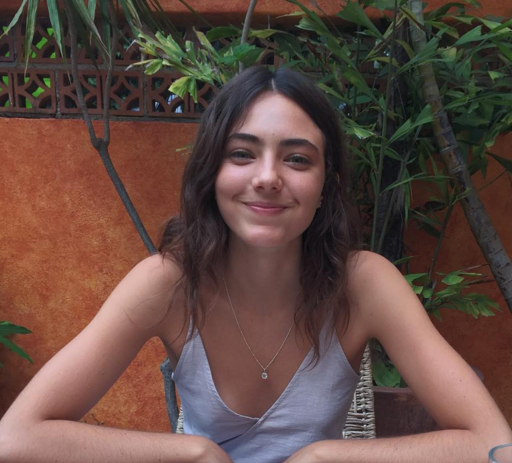
\includegraphics[width=2.5in]{images/expt3/1e.png}
		}
		\hspace{0.2in}
\subfigure[Right image]{
	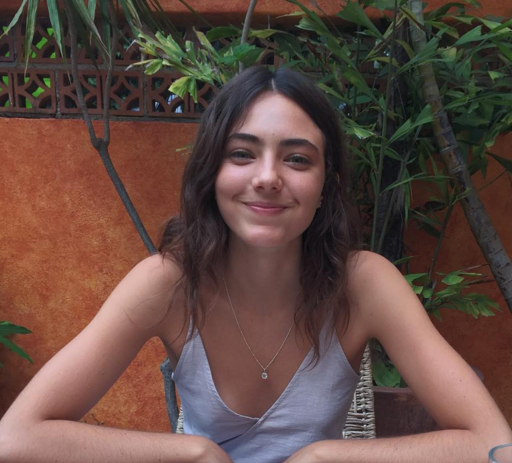
\includegraphics[width=2.5in]{images/expt3/1f.png}
		}
\caption [Dirty images,  Shepp-Logan phantom, Left 30 lines, Right 20 lines, rms $1e^{-4}$]{Dirty images, Shepp-Logan phantom, Left 30 lines, Right 20 lines, rms $1e^{-4}$}
\label{fig:expt33}
%\end{center}
\end{figure}
\item The relative error vs.  $\lambda$ graphs for the left and right images are shown in Fig. \ref{fig:expt34}.

\begin{figure}[H]

%\begin{center}  \vspace{-0.1in}
\subfigure[Left image]{
	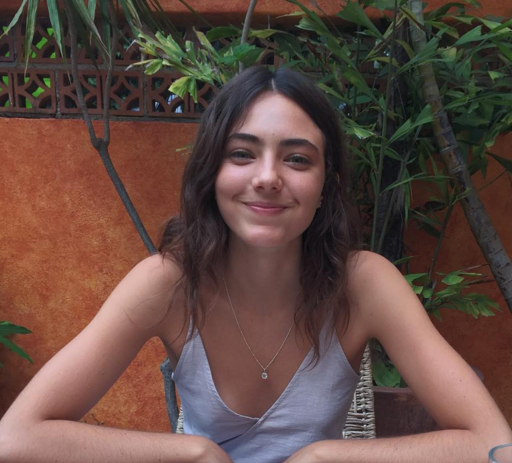
\includegraphics[width=3in]{images/expt3/2a.png}
		}
\hspace{-0.1in}
\subfigure[Right image]{
	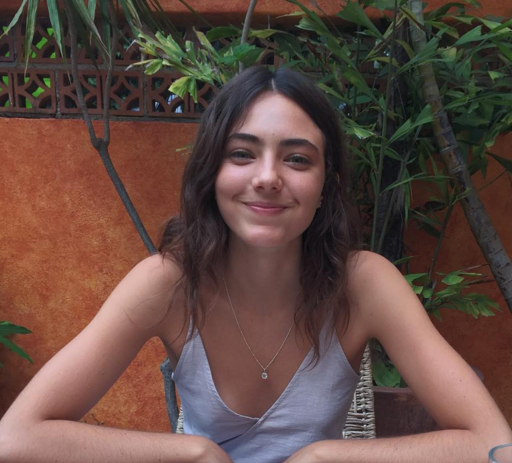
\includegraphics[width=2.9in]{images/expt3/2b.png}
		}
\caption [Error vs $\lambda$, Shepp-Logan phantom, 50\% overlap,  Left 30 lines, Right 20 lines, rms $1e^{-4}$]{Error vs $\lambda$, Shepp-Logan phantom, 50\% overlap,  Left 30 lines, Right 20 lines, rms $1e^{-4}$}
\label{fig:expt34}
%\end{center}
\end{figure}

\item The reconstructed left and right images for $\lambda = 1e^{-3.5}$ for  $\mu  = 0.1 $  and $\lambda = 1e^{-2}$ for  $\mu = 0$ are shown in Fig. \ref{fig:expt35} and  Fig. \ref{fig:expt36} respectively. 

\vspace{-0.2in}
\begin{figure}[t!]
\hspace{0.4in}
%\begin{center}  \vspace{-0.1in}
\subfigure[Coupled, $\mu = 0.01, \lambda = 1e^{-3.5}$]{
	\includegraphics[width=2.5in]{images/expt3/4b.png}
		}
\hspace{0.2in}
\subfigure[Separate, $\mu = 0, \lambda = 1e^{-2}$]{
	\includegraphics[width=2.5in]{images/expt3/4a.png}
		}		
\caption [Reconstructed left images, Shepp-Logan phantom, 50\% overlap,  Left 30 lines, Right 20 lines, rms $1e^{-4}$]{Reconstructed left images, Shepp-Logan phantom, 50\% overlap,  Left 30 lines, Right 20 lines, rms $1e^{-4}$}
\label{fig:expt35}
%\end{center}
\end{figure}

\vspace{-0.2in}
\begin{figure}[b!]
\hspace{0.4in}
%\begin{center}  \vspace{-0.1in}
\subfigure[Coupled, $\mu = 0.01, \lambda = 1e^{-3.5}$]{
	\includegraphics[width=2.5in]{images/expt3/3b.png}
		}
\hspace{0.2in}
\subfigure[Separate, $\mu = 0, \lambda = 1e^{-1.5}$]{
	\includegraphics[width=2.5in]{images/expt3/3a.png}
		}		
\caption [Reconstructed right images, Shepp-Logan phantom, 50\% overlap,  Left 30 lines, Right 20 lines, rms $1e^{-4}$]{Reconstructed right images, Shepp-Logan phantom, 50\% overlap,  Left 30 lines, Right 20 lines, rms $1e^{-4}$. The reconstruction using coupled formulation is visually much better}
\label{fig:expt36}
%\end{center}
\end{figure}
\end{enumerate}
\newpage
\subsubsection{Observations}

\begin{enumerate}
\item From the error graphs and the reconstructed images we observe that for both left and right images the alternating algorithm using the coupled formulation performs better than the uncoupled formulation
\item For the best value of $\lambda$ for the left image the error improves from approximately 0.114 to approximately 0.105 by using coupling and for the right image the error improves from approximately 0.221 to approximately 0.142.
\item For the right image for which we have Fourier data only on 20 sampling lines the improvement is clearly pronounced.
\item This is because the left image has Fourier data available on 30 sampling lines and thus we expect the uncoupled reconstruction of the left image to better than that of the right image. By introducing the coupling term this is transferred into the right image also and we get significant improvement in performance.
\item For the left image the improvement by using the coupled formulation is not as pronounced as that for the right image.
\end{enumerate}

\subsubsection{Experiment with 35 and 25 sampling lines}

\begin{enumerate}
\item We conduct the same experiment as above with the only the sampling maps changed.
\item Fourier data is availabe at locations given by the sampling map which consist of 35 lines (12170 points) and 25 lines (8808 points) respectively for the left and right image as shown in Fig. \ref{fig:expt37}
\begin{figure}[b!]

\hspace{-0.5in}
%\begin{center}  \vspace{-0.1in}
\subfigure[Left image]{
	\includegraphics[width=4in]{images/expt3/5a.png}
		}
		\hspace{-1in}
\subfigure[Right image]{
	\includegraphics[width=4in]{images/expt3/5b.png}
		}
\caption [Sampling maps, Left 35 lines, Right 25 lines]{Sampling maps, Left 35 lines, Right 25 lines}
\label{fig:expt37}
%\end{center}
\end{figure}
\item We choose $\mu = 0, \mu = 0.01$ and $\mu = 0.1$ where in the first case there is no coupling and in the latter two cases coupling is present. We use $\lambda_x = \lambda_y = \lambda$ and vary it in the logarithmic scale between [-4, -2] in steps of size 0.5. 

\begin{figure}[h!]

\vspace{-0.2in}
%\begin{center}  \vspace{-0.1in}
\subfigure[Left image]{
	\includegraphics[width=3in]{images/expt3/6a.png}
		}
\hspace{-0.1in}
\subfigure[Right image]{
	\includegraphics[width=3in]{images/expt3/6b.png}
		}
\caption [Error vs $\lambda$, Shepp-Logan phantom, 50\% overlap,  Left 35 lines, Right 25 lines, rms $1e^{-4}$]{Error vs $\lambda$, Shepp-Logan phantom, 50\% overlap,  Left 35 lines, Right 25 lines, rms $1e^{-4}$}
\label{fig:expt38}
%\end{center}
\end{figure}
\item The relative error vs.  $\lambda$ graphs for the left and right images are shown in Fig. \ref{fig:expt38}.
\item The reconstructed left and right images for $\lambda = 1e^{-3.5}$ for  $\mu  = 0.1 $  and $\lambda = 1e^{-2}$ for  $\mu = 0$ are shown in Fig. \ref{fig:expt39} and  Fig. \ref{fig:expt310} respectively. 


\begin{figure}[b!]
\hspace{0.4in}
%\begin{center}  \vspace{-0.1in}
\subfigure[Coupled, $\mu = 0.01, \lambda = 1e^{-3.5}$]{
	\includegraphics[width=2.5in]{images/expt3/7a.png}
		}
\hspace{0.2in}
\subfigure[Separate, $\mu = 0, \lambda = 1e^{-2}$]{
	\includegraphics[width=2.5in]{images/expt3/7b.png}
		}		
\caption [Reconstructed left images, Shepp-Logan phantom, 50\% overlap,  Left 35 lines, Right 25 lines, rms $1e^{-4}$]{Reconstructed left images, Shepp-Logan phantom, 50\% overlap,  Left 35 lines, Right 25 lines, rms $1e^{-4}$}
\label{fig:expt39}
%\end{center}
\end{figure}


\begin{figure}[t!]
\hspace{0.4in}
%\begin{center}  \vspace{-0.1in}
\subfigure[Coupled, $\mu = 0.01, \lambda = 1e^{-3.5}$]{
	\includegraphics[width=2.5in]{images/expt3/8a.png}
		}
\hspace{0.2in}
\subfigure[Separate, $\mu = 0, \lambda = 1e^{-1.5}$]{
	\includegraphics[width=2.5in]{images/expt3/8b.png}
		}		
\caption [Reconstructed right images, Shepp-Logan phantom, 50\% overlap,  Left 35 lines, Right 25 lines, rms $1e^{-4}$]{Reconstructed right images, Shepp-Logan phantom, 50\% overlap,  Left 35 lines, Right 25 lines, rms $1e^{-4}$. The reconstruction using the coupled framework is better than the other.}
\label{fig:expt310}
%\end{center}
\end{figure}
\end{enumerate}

\subsubsection{Observations}

\begin{enumerate}
\item From the error graphs and the reconstructed images we observe that for both left and right images the alternating algorithm using the coupled formulation performs better than the uncoupled formulation
\item For the best value of $\lambda$ for the left image the error improves from approximately 0.081 to 0.071 by using coupling and for the right image the error improves from approximately 0.152 to 0.094.
\item Again for the right image the improvement is more pronounced than that for the left image due to the fact that for the left image we have Fourier data on 35 sampling lines and for the right image we have Fourier data only on 25 sampling lines.
\item   Since we expect the higher number of samples for the left image to lead to a better reconstruction in the uncoupled formulation, this higher quality is transferred to the right image when we introduce coupling.
\item Comparing the relative error graphs in Fig. \ref{fig:expt38} and Fig. \ref{fig:expt34} we observe that the percentage improvement in the error reduces as data at higher number of Fourier points is available. This conforms with the intuition that if we have almost all Fourier measurements, then we expect both the coupled and uncoupled formulation to perform almost similarly. 
\item We will not deal with radio astronomical extended sources separately in this section but instead will combine the extended sources with point sources and investigate them in the next section.
\end{enumerate}


\section{Experiments on images containing both point and extended sources}
\begin{enumerate}
\item In this section we consider images that consist of both point and extended sources. It is unlikely to find a region of the sky with extended sources alone and most likely we will find extended sources along with point sources in the background. In this case our image will not be sparse in any one domain and we must come up with an alternate formulation to reconstruct such images from incomplete fourier data.
\item Let $J$ be the image containing both point sources and extended sources. We can view $J$ as the sum of two images $J_s$ and $J_w$ where, $J_s$ refers to the image of point source and is sparse in spatial domain and $J_w$ refers to image containing the extended source and is sparse in wavelet domain. An example of such a decomposition is given in Fig. \ref{fig:expt41}.
\item We have,
\begin{eqnarray}
J_w &=& W u \\
J_s &=& I v,
\end{eqnarray}
where  $u$ denotes the wavelet coefficieints, $v$ denotes the pixel values, $W$ refers to the matrix representing the inverse wavelet transform and $I$ refers to the identity matrix.
\begin{figure}[b!]
\hspace{0.4in}
%\vspace{-0.2in}
%\begin{center}  \vspace{-0.1in}
\subfigure[Complete image]{
	\includegraphics[width=1.7in]{images/expt4/1a.png}
		}
\hspace{0.1in}
\subfigure[Spatial domain sparse]{
	\includegraphics[width=1.7in]{images/expt4/1b.png}
		}
		\hspace{0.1in}
\subfigure[Wavelet sparse]{
	\includegraphics[width=1.7in]{images/expt4/1c.png}
		}
\caption [Decomposition of image containing both point and extended sources]{Decomposition of image containing both point and extended sources}
\label{fig:expt41}
%\end{center}
\end{figure}
\item Thus we have,
\begin{equation}
	J = W u + I v.
\end{equation} 
\item Now let us consider a setting as before where we have two images with some information overlap. Let the lexicographic ordering of the left image be denoted by $x$ of size $N \times 1$ and that of the right image by denoted by $y$ of size $N \times 1$. Then,
\begin{eqnarray}
	x &=& Wu_x + Iv_x \\
	y  &=& Wu_y + Iv_y	
\end{eqnarray}
\item We have Fourier measurements $b_x$ and $b_y$ using the sampling matrices $\Phi_x$ and $\Phi_y$ where,
	\begin{eqnarray}
  b_x &=& \Phi_x x  + n_x\\
  b_y   &=& \Phi_y y + n_y,
  \end{eqnarray}
 where $\Phi_x$ and $\Phi_y$ are $M_x \times N$ and $M_y \times N$ measurement matrices respectivley and $n_x$ and $n_y$ are terms corresponding to the noise added to the system while obtaining the measurements ($M_x < N, \ M_y < N)$.
 
\item Let $f_x$ and $f_y$ be the $S \times 1$ feature vectors obtained from $x$ and $y$ as,
\begin{eqnarray}
f_x &=& B_x u_x + C_x v_x\\
f_y &=& B_y u_y + C_y v_y,
\label{eq:mix}
\end{eqnarray}
where $B_x, B_y, C_x$ and $C_y$ are feature extraction matrices.

\item Then along the lines of Formulation-3 we will find $u_x^*, v_x^*, u_y^* and v_y^*$ by performing joint minimization of the cost function $G(u_x, v_x, u_y, v_y)$ as follows:
 \begin{equation}
u_x^*, v_x^*, u_y^*, v_y^* = \arg \min_{u_x, v_x, u_y, v_y} G(u_x, v_x, u_y, v_y)
 \end{equation}
where,
 \begin{eqnarray}
G(u_x, v_x, u_y, v_y) &\equiv& \|\Phi_x\Psi u_x + \Phi v_x - b_x\|_2^2 + \|\Phi_y\Psi u_y +\Phi v_y  - b_y\|_2^2 + \lambda^s_x \|u_x\|_1 + \lambda^w_x \|v_x\|_1 \nonumber \\
& & +  \lambda^s_y \|u_y\|_1 + \lambda^w_y \|v_y\|_1   + \mu ||f_x - f_y||_2^2.
\label{eq:cstf}
 \end{eqnarray}
\item Here $\lambda^s_x$ and $\lambda^s_y$ are weights to the spatial domain sparse component of the reconstructed image while $\lambda^w_x$ and $\lambda^w_y$ are weights to the wavelet domain sparse component. In general these can be different since we may have a different level of sparsity in the two domains.
\item We will make the simplifying assumption and choose $\lambda^s_x = \lambda^w_x = \lambda_x$ and $\lambda^s_y = \lambda^w_y = \lambda_y$.
\item Under this assumption we can express the above minimization problem using Formulation-3 where,
\begin{align}
z_x &= \begin{bmatrix}
u_x \\
v_x
\end{bmatrix}\\
z_y &= \begin{bmatrix}
u_y \\
v_y
\end{bmatrix}\\
A_x &= \begin{bmatrix}
\Phi_x\Psi &  \Phi_x
\end{bmatrix}\\
A_y &= \begin{bmatrix}
\Phi_y\Psi &  \Phi_y
\end{bmatrix}\\
D_x &= \begin{bmatrix}
B_x &  0 \\
0 & C_x
\end{bmatrix}\\
D_y &= \begin{bmatrix}
B_y &  0 \\
0 & C_y
\end{bmatrix}
\end{align}
\item Thus we will first find $z_x^*$ and $z_y^*$ by solving the joint minimization problem,
 \begin{equation}
 z_x^*, z_y^* = \arg \min_{z_x, z_y} F(z_x, z_y),
 \end{equation}
where,
 \begin{equation}
 F(z_x, z_y) \equiv \|A_x z_x - b_x\|_2^2 + \|A_y z_y - b_y\|_2^2 + \lambda_x \|z_x\|_1 + \lambda_y \|z_y\|_1 + \mu ||D_x z_x - D_y z_y||_2^2.
 \end{equation}
\end{enumerate}
We conduct three classes of experiments with this formulation,
\begin{enumerate}
\item Experiment to confirm the need of a better description for images consisting of both point and extended sources
\item Images consisting of both the Shepp-Logan phantom and point sources. The Shepp-Logan phantom is a prime example of a wavelet sparse image and hence we use this to test our framework.
\item Images consisting of both astronomical point sources and astronomical extended sources.
\end{enumerate}

\subsection{Experiment to confirm need for better description}

\begin{enumerate}
\item In this experiment we will consider a single image reconstruction problem where the image consists of a spatial domain sparse component and a wavelet domain sprase component. We will perform the reconstruction using both the formulation presented above and a formulation that considers the image only to be wavelet sparse. In both cases we will make use of the FISTA algorithm to perform the reconstruction. It is clear that a formulation that considers the image to be sparse in spatial domain will certainly not work so we dont consider that case.
\item We construct the original image by adding 100 stars at random locations in the background of the Shepp-Logan phantom image as shown in Fig. \ref{fig:expt42}. Each star is of size $2\times2$ pixels and has uniform intensity value of 1.

 \begin{figure}[t!]
	\centering \vspace{-0.1in}
	\includegraphics[width=2.5in]{images/expt4/2.png}
	 \caption[Original image, Shepp-Logan phantom, 100 stars ]{\small Original image, Shepp-Logan phantom, 100 stars}
	\label{fig:expt42}
\end{figure}


\item We have Fourier data according to the sampling map consisting of 35 sampling lines (12170 points points) as shown in Fig. \ref{fig:expt43}.
 \begin{figure}[t!]
	\centering 
	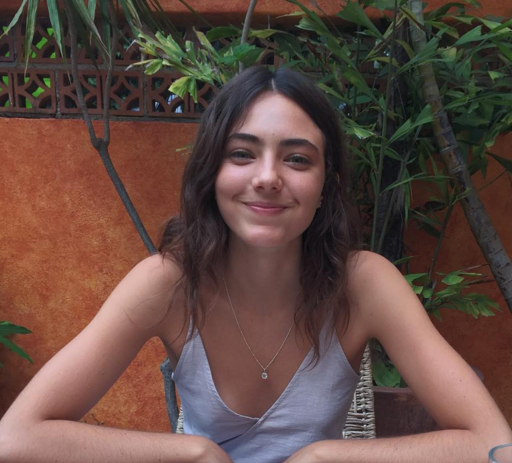
\includegraphics[width=2.2in]{images/expt4/3.png}
	 \caption[Sampling map, 35 lines ]{\small Sampling map, 35 lines}
	\label{fig:expt43}
\end{figure}
\item We assume that there is no noise.
\item The Lipschitz constants $L$ is determined as:
\begin{eqnarray}
L &=& 2\max(eig( A^T A) 
\end{eqnarray}
This value can be upper bounded by $4$.
\item The value of $\lambda$ is varied in the logarithmic scale between [-4, 0] in steps of 0.5.
 \begin{figure}[b!]
	\centering \vspace{-0.1in}
	\includegraphics[width=2.5in]{images/expt4/4.png}
	 \caption[Dirty image, Shepp-Logan phantom, 100 stars, 35 lines ]{\small Dirty image, Shepp-Logan phantom, 100 stars, 35 lines}
	\label{fig:expt44}
\end{figure}
\item From the dirty image (Fig. \ref{fig:expt44}) it is not easy to recover the coefficients of the wavelet domain sparse and spatial domain sparse component. But since our algorithm is insensitive to starting point we initialize both sets of coefficients with the corresponding coefficients derived from the combined image.


\item The error vs $\lambda$ plot for the two formulations is shown in Fig. \ref{fig:expt45}.

 \begin{figure}[t!]
	\centering \vspace{-0.1in}
	\includegraphics[width=3.5in]{images/expt4/5.png}
	 \caption[Error vs $\lambda$, Shepp-Logan phantom, 100 stars, 35 lines ]{\small Error vs $\lambda$, Shepp-Logan phantom, 100 stars, 35 lines}
	\label{fig:expt45}
\end{figure}


\item The reconstructed image for the best value of $\lambda$ using the formulation presented above and the formulation that assumes the image to be sparse in wavelet domain alone is shown in Fig. \ref{fig:expt46}.
\begin{figure}[b!]
\hspace{0.4in}
%\begin{center}  \vspace{-0.1in}
\subfigure[Sum of wavelet sparse and spatial domain sparse, $\lambda = 1e^{-2}$]{
	\includegraphics[width=2.5in]{images/expt4/6a.png}
		}
\hspace{0.2in}
\subfigure[Wavelet domain sparse only, $\lambda = 1e^{-2}$]{
	\includegraphics[width=2.5in]{images/expt4/6b.png}
		}		
\caption [Reconstructed images, Shepp-Logan phantom, 100 stars]{Reconstructed images, Shepp-Logan phantom, 100 stars. The reconstruction of the phantom is better in the left image}
\label{fig:expt46}
%\end{center}
\end{figure}


\item The spatial domain sparse component and the wavelet domain sparse component of the reconstruction using the new formulation is shown in Fig. \ref{fig:expt47}.
\begin{figure}[t!]
\hspace{0.4in}
%\begin{center}  \vspace{-0.1in}
\subfigure[Spatial domain sparse]{
	\includegraphics[width=2.5in]{images/expt4/7a.png}
		}
\hspace{0.2in}
\subfigure[Wavelet domain sparse]{
	\includegraphics[width=2.5in]{images/expt4/7b.png}
		}		
\caption [Reconstructed image decompositions, Shepp-Logan phantom, 100 stars, $\lambda = 1e^{-2}$ ]{Reconstructed image decompositions, Shepp-Logan phantom, 100 stars, $\lambda = 1e^{-2}$}
\label{fig:expt47}
%\end{center}
\end{figure}
\end{enumerate}


\subsubsection{Observations}
\begin{enumerate}
\item The formulation that assumes the image to be only wavelet sparse performs much worse than the formulation that considers the image to have both a spatial domain sparse component and a wavelet domain sparse component.
\item The spatial domain sparse component of the reconstructed image consists of not only the point sources but also parts of the edges of the Shepp-Logan phantom. This is to be expected since the edges have high contribution to the wavelet coefficients in the wavelet domain sparse image.
\item The wavelet domain sparse component contains the Shepp-Logan phantom and also a few stray stars.
\item Thus we need the formulation presented above to tackle images that contain both a spatial domain sparse component and a wavelet domain sparse component.
\end{enumerate}

\subsection{Experiments on images of Shepp-Logan phantom along with stars}
In this section we will use the formulation above to reconstruct left and right images where there is information overlap between the two images. We compare the performance of the cases where we do joint minimization using the alternating algorithms with the case where we solve for left and right images separately. By decomposing the image into two components (a wavelet domain sparse component and a spatial domain sparse component) we are effectively increasing the size of the problem by a factor of 2 and to obtain faster run times we use the FISTA variant of the alternating algorithm.
\subsubsection{Experiment with 40 sampling lines for both images}
\begin{enumerate}
\item The left image is constructed as follows. We start with the Shepp-Logan phantom and add 200 stars at random locations in the background. Each star is of size $2 \times 2$ pixels and has intensity value of 1.
\item For the right image, we start with the same Shepp-Logan phantom image and add 200 stars in different random locations as compared to the left image. The two original images are shown in Fig. \ref{fig:expt51}.
\item Thus the two images can be viewed as having a common wavelet sparse component and different spatial domain sparse components.
\begin{figure}[b!]
\hspace{0.4in}
%\begin{center}  \vspace{-0.1in}
\subfigure[Left image]{
	\includegraphics[width=2.5in]{images/expt5/1a.png}
		}
		\hspace{0.2in}
\subfigure[Right image]{
	\includegraphics[width=2.5in]{images/expt5/1b.png}
		}
\caption [Original images, Shepp-Logan phantom, 200 stars]{Original images, Shepp-Logan phantom, 200 stars. Only the star locations in both images are different}
\label{fig:expt51}
%\end{center}
\end{figure}

\item Fourier data is available at locations given by the sampling map which consist of 40 lines (13387 points) for voth the left and right image as shown in Fig. \ref{fig:expt52}
\begin{figure}[!t]

\begin{center}  \vspace{-0.1in}

\includegraphics[width=2.5in]{images/expt5/2.png}

\caption [Sampling map, 40 lines]{Sampling map, 40 lines}
\label{fig:expt52}
\end{center}
\end{figure}

\item We consider the noiseless case. The information overlap present is that the wavelet sparse component of both images must be the same. Thus in Eq. \ref{eq:mix}, we have, $B_x = W, C_x = 0, B_y = W$ and $C_y = 0$ where $W$ is the inverse wavelet transform operator. 
\item From the dirty images (Fig. \ref{fig:expt53}) it is not easy to recover the coefficients of the wavelet domain sparse and spatial domain sparse component. But since our algorithm is insensitive to starting point we initialize both sets of coefficients with the corresponding coefficients derived from the combined images.

\begin{figure}[!b]
\hspace{0.4in}
%\begin{center}  \vspace{-0.1in}
\subfigure[Left image]{
	\includegraphics[width=2.5in]{images/expt5/3a.png}
		}
		\hspace{0.2in}
\subfigure[Right image]{
	\includegraphics[width=2.5in]{images/expt5/3b.png}
		}
\caption [Dirty images,  Shepp-Logan phantom, 200 stars, 40 lines]{Dirty images,  Shepp-Logan phantom, 200 stars, 40 lines}
\label{fig:expt53}
%\end{center}
\end{figure}

\item We choose $\mu = 0$ and $\mu = 0.1$ where in the first case there is no coupling and in the latter case coupling is present. We use $\lambda_x = \lambda_y = \lambda$ and vary it in the logarithmic scale between [-5.5, -3] in steps of size 0.5. 
\item The Lipschitz constant in this case can be upper bounded by $2(2 + \mu)$.
\item We terminate the algorithm either when the relative difference in value of objective function is less than $1e^{-7}$ or when we reach 20000 iterations.


\item The relative error vs.  $\lambda$ graphs for the left and right images are shown in Fig. \ref{fig:expt54}.

\begin{figure}[H]

%\begin{center}  \vspace{-0.1in}
\subfigure[Left image]{
	\includegraphics[width=3.2in]{images/expt5/4a.png}
		}
\hspace{-0.1in}
\subfigure[Right image]{
	\includegraphics[width=3.2in]{images/expt5/4b.png}
		}
\caption [Error vs $\lambda$, Shepp-Logan phantom, 200 stars,  40 lines]{Error vs $\lambda$, Shepp-Logan phantom, 200 stars,  40 lines]}
\label{fig:expt54}
%\end{center}
\end{figure}

\item The reconstructed left and right images for $\lambda = 1e^{-5}$ for  $\mu  = 0.1 $  and $\lambda = 1e^{-5}$ for  $\mu = 0$ are shown in Fig. \ref{fig:expt55} and  Fig. \ref{fig:expt56} respectively. 

\vspace{-0.2in}
\begin{figure}[H]
\hspace{0.4in}
%\begin{center}  \vspace{-0.1in}
\subfigure[Coupled, $\mu = 0.1, \lambda = 1e^{-5}$]{
	\includegraphics[width=2.5in]{images/expt5/5a.png}
		}
\hspace{0.2in}
\subfigure[Separate, $\mu = 0, \lambda = 1e^{-5}$]{
	\includegraphics[width=2.5in]{images/expt5/5b.png}
		}		
\caption [Reconstructed left images, Shepp-Logan phantom, 200 stars, 40 lines]{Reconstructed left images, Shepp-Logan phantom, 200 stars, 40 lines. The reconstruction of the phantom is visibly better in the coupled formulation.}
\label{fig:expt55}
%\end{center}
\end{figure}


\begin{figure}[H]
\hspace{0.4in}
%\begin{center}  \vspace{-0.1in}
\subfigure[Coupled, $\mu = 0.1, \lambda = 1e^{-5}$]{
	\includegraphics[width=2.5in]{images/expt5/6a.png}
		}
\hspace{0.2in}
\subfigure[Separate, $\mu = 0, \lambda = 1e^{-5}$]{
	\includegraphics[width=2.5in]{images/expt5/6b.png}
		}		
\caption [Reconstructed right images, Shepp-Logan phantom, 200 stars, 40 lines]{Reconstructed right images, Shepp-Logan phantom, 200 stars, 40 lines. The reconstruction of the phantom is visibly better in the coupled formulation.}
\label{fig:expt56}
%\end{center}
\end{figure}
\end{enumerate}
\subsubsection{Observations}
\begin{enumerate}
\item From the error graphs and the reconstructed images we observe that for both left and right images the alternating algorithm using the coupled formulation performs better than the uncoupled formulation
\item For the best value of $\lambda$ for the left image the error improves from approximately 0.102 to 0.056 by using coupling and for the right image the error improves from approximately 0.105 to 0.056.
\item Since the level of sparsity in both images and the sampling points are the same in both images both the error and the improvement in error are similar in left and right images.
\end{enumerate}

We also performed the experiment where the sampling map for the left image consisted of 40 sampling lines and that of the right image consisted of 30 sampling lines. In this case, we observed that the improvement in the reconstruction of the right image which has fewer number of sampling points is much higher than that in the reconstruction of the left image. This is due to the fact that for the right image, the uncoupled formulation performs much worse as compared to for the left image since it has Fourier data available at much fewer points.
%
%\subsubsection{Experiment with 40 sampling lines for left image and 30 sampling lines for the right image}
%\begin{enumerate}
%\item We repeat the above experiment but this time we consider the case where Fourier data is available on 40 sampling lines for the left image and only on 30 sampling lines for the right image.
%\item The original images in this case will have stars at different random locations as compared to the previous experiment but we keep rest of the parameters and settings the same as in the above experiment.
%\item The relative error vs.  $\lambda$ graphs for the left and right images are shown in Fig. \ref{fig:expt57}.
%
%\begin{figure}[H]
%
%%\begin{center}  \vspace{-0.1in}
%\subfigure[Left image]{
%	\includegraphics[width=3.2in]{images/expt5/7a.png}
%		}
%\hspace{-0.1in}
%\subfigure[Right image]{
%	\includegraphics[width=3.2in]{images/expt5/7b.png}
%		}
%\caption [Error vs $\lambda$, Shepp-Logan phantom, 200 stars,  Left 40 lines, Right 30 lines]{Error vs $\lambda$, Shepp-Logan phantom, 200 stars,  Left 40 lines, Right 30 lines]}
%\label{fig:expt57}
%%\end{center}
%\end{figure}
%
%\item The reconstructed left and right images for $\lambda = 1e^{-5}$ for  $\mu  = 0.1 $  and $\lambda = 1e^{-5}$ for  $\mu = 0$ are shown in Fig. \ref{fig:expt58} and  Fig. \ref{fig:expt59} respectively. 
%
%\vspace{-0.2in}
%\begin{figure}[H]
%
%%\begin{center}  \vspace{-0.1in}
%\subfigure[Coupled, $\mu = 0.1, \lambda = 1e^{-5}$]{
%	\includegraphics[width=2.5in]{images/expt5/8a.png}
%		}
%\hspace{0.2in}
%\subfigure[Separate, $\mu = 0, \lambda = 1e^{-5}$]{
%	\includegraphics[width=2.5in]{images/expt5/8b.png}
%		}		
%\caption [Reconstructed left images, Shepp-Logan phantom, 200 stars, Left 40 lines,  Right 30 lines]{Reconstructed left images, Shepp-Logan phantom, 200 stars, Left 40 lines,  Right 30 lines}
%\label{fig:expt58}
%%\end{center}
%\end{figure}
%
%
%\begin{figure}[H]
%
%%\begin{center}  \vspace{-0.1in}
%\subfigure[Coupled, $\mu = 0.1, \lambda = 1e^{-5}$]{
%	\includegraphics[width=2.5in]{images/expt5/9a.png}
%		}
%\hspace{0.2in}
%\subfigure[Separate, $\mu = 0, \lambda = 1e^{-5}$]{
%	\includegraphics[width=2.5in]{images/expt5/9b.png}
%		}		
%\caption [Reconstructed right images, Shepp-Logan phantom, 200 stars, Left 40 lines,  Right 30 lines]{Reconstructed right images, Shepp-Logan phantom, 200 stars, Left 40 lines,  Right 30 lines}
%\label{fig:expt59}
%%\end{center}
%\end{figure}
%\end{enumerate}
%\subsubsection{Observations}
%\begin{enumerate}
%\item From the error graphs and the reconstructed images we observe that for both left and right images the alternating algorithm using the coupled formulation performs better than the uncoupled formulation
%\item For the best value of $\lambda$ for the left image the error improves from approximately 0.10 to 0.06 by using coupling and for the right image the error improves from approximately 0.20 to 0.08.
%\item For the right image the improvement is more pronounced than that for the left image due to the fact that for the left image we have Fourier data on 40 sampling lines and for the right image we have Fourier data only on 30 sampling lines.
%\item  Thus the gains of using the coupled formulation are much higher when we have higher number of samples for one image and lower number of samples for the other image. In this case, the reconstruction of the image with the lower number of samples is improved significantly.
%\end{enumerate}
In the next section, we will consider images of extended astronomical sources along with point sources and conduct experiments to investigate the performance using the coupled formulation.

\subsection{Experiment on images containing astronomical extended and point sources}
In this section we will explore the case where a large difference in the number of sampling points present in the left and right images may lead to loss in performance in the image with the higher number of samples while using the coupled framework.
We will refer to this problem as the ``difference in sampling points problem'' and will subsequently present 3 different ways to tackle this problem.
\begin{enumerate}
\item The original left and right images shown in Fig. \ref{fig:expt61} and consist of an extended source along with 200 stars.
There is an overlap of 128 columns between the two images.
\item The stars are of size $2 \times 2$ and have intensity values in range [0.3, 1] picked uniform randomly.
\item Fourier data is available at the sampling maps generated by the GMRT array using aperture synthesis as shown in Fig. \ref{fig:expt62}.

\item For the left image, we consider sampling map generated by aperture synthesis for 12 hours with a sample collected every 10 minutes.
\item For the left image, we consider sampling map generated by aperture synthesis for 12 hours with a sample collected every 30 minutes.
\item There is a large difference in the number of points in the sampling map of the left and right images. The left sampling map has 23884 points while the right sampling map has 11192.
\begin{figure}[h!]
\hspace{0.4in}
%\begin{center}  \vspace{-0.1in}
\subfigure[Left image]{
	\includegraphics[width=2.5in]{images/expt6/1a.png}
		}
		\hspace{0.2in}
\subfigure[Right image]{
	\includegraphics[width=2.5in]{images/expt6/1b.png}
		}
\caption [Original images, Extended source, 200 stars]{Original images, Extended source , 200 stars. Overlap of 128 columns}
\label{fig:expt61}
%\end{center}
\end{figure}

\begin{figure}[h!]

\hspace{0.4in}
%\begin{center}  \vspace{-0.1in}
\subfigure[Left image, Sampling period = 10 min]{
	\includegraphics[width=2.5in]{images/expt6/2a.png}
		}
		\hspace{0.2in}
\subfigure[Right image, Sampling period = 30 min]{
	\includegraphics[width=2.5in]{images/expt6/2b.png}
		}
\caption [Sampling maps, Duration = 12h]{Sampling maps, Duration = 12h}
\label{fig:expt62}
%\end{center}
\end{figure}

\item The extended source forms the wavelet sparse component (approx. 3700 significant coefficients) of our image and the stars form the spatial domain sparse component. A coefficient is said to be significant if it is more than 0.5\% of maximum coefficient value.

\item The information overlap that we assume is that the last 128 columns of the wavelet sparse component of the left image match with the first 128 columns of the wavelet sparse component of the right image.
\item We could in general assume overlap for the spatial domain sparse components too but we do not consider this.
\item We consider the noiseless case. We initialize both sets of coefficients with the corresponding coefficients derived from the dirty images shown in Fig. \ref{fig:expt63}.
%\begin{center}  \vspace{-0.1in}

\begin{figure}[h!]
\hspace{0.4in}
\subfigure[Left image, Sampling period = 10 min]{
	\includegraphics[width=2.5in]{images/expt6/3a.png}
		}
		\hspace{0.2in}
\subfigure[Right image, Sampling period = 30 min]{
	\includegraphics[width=2.5in]{images/expt6/3b.png}
		}
\caption [Dirty images, Extended source, 200 stars, Duration 12h]{Dirty images, Extended source , 200 stars, Duration 12h}
\label{fig:expt63}
%\end{center}
\end{figure}


\item We choose $\mu = 0$ and $\mu = 0.1$ where in the first case there is no coupling and in the latter case coupling is present. We use $\lambda_x = \lambda_y = \lambda$ and vary it in the logarithmic scale between [-6, -2] in steps of size 0.5. 
\item The Lipschitz constant in this case can be upper bounded by $2(2 + \mu)$.
\item We terminate the algorithm either when the relative difference in value of objective function is less than $1e^{-7}$ or when we reach 20000 iterations.
\item The relative error vs.  $\lambda$ graphs for the left and right images are shown in Fig. \ref{fig:expt64}.

\begin{figure}[h!]

%\begin{center}  \vspace{-0.1in}
\subfigure[Left image]{
	\includegraphics[width=3.2in]{images/expt6/4a.png}
		}
\hspace{-0.1in}
\subfigure[Right image]{
	\includegraphics[width=3.2in]{images/expt6/4b.png}
		}
\caption [Error vs $\lambda$, Extended source, 200 stars,  Duration = 12h, Left sampling period = 10 min, Right sampling period = 30 min]{Error vs $\lambda$, Extended source, 200 stars,  Duration = 12h, Left sampling period = 10 min, Right sampling period = 30 min}
\label{fig:expt64}
%\end{center}
\end{figure}

\item The reconstructed left and right images for $\lambda = 1e^{-5}$ for  $\mu  = 0.1 $  and $\lambda = 1e^{-5}$ for  $\mu = 0$ are shown in Fig. \ref{fig:expt65} and  Fig. \ref{fig:expt66} respectively. 

\begin{figure}[H]
\hspace{0.4in}
%\begin{center}  \vspace{-0.1in}
\subfigure[Coupled, $\mu = 0.1, \lambda = 1e^{-3}$]{
	\includegraphics[width=2.5in]{images/expt6/5a.png}
		}
\hspace{0.2in}
\subfigure[Separate, $\mu = 0, \lambda = 1e^{-3}$]{
	\includegraphics[width=2.5in]{images/expt6/5b.png}
		}		
\caption [Left reconstructed images , Extended source, 200 stars,  Duration = 12h, Left sampling period = 10 min, Right sampling period = 30 min]{Left reconstructed images, Extended source, 200 stars,  Duration = 12h, Left sampling period = 10 min, Right sampling period = 30 min}
\label{fig:expt65}
%\end{center}
\end{figure}

\begin{figure}[H]
\hspace{0.4in}
%\begin{center}  \vspace{-0.1in}
\subfigure[Coupled, $\mu = 0.1, \lambda = 1e^{-3}$]{
	\includegraphics[width=2.5in]{images/expt6/6a.png}
		}
\hspace{0.2in}
\subfigure[Separate, $\mu = 0, \lambda = 1e^{-2}$]{
	\includegraphics[width=2.5in]{images/expt6/6b.png}
		}		
\caption [Right reconstructed images , Extended source, 200 stars,  Duration = 12h, Left sampling period = 10 min, Right sampling period = 30 min]{Right  reconstructed images, Extended source, 200 stars,  Duration = 12h, Left sampling period = 10 min, Right sampling period = 30 min. The reconstructed image using the separate formulation has excess stars in bottom right. The features in the left of the extended sources are clearer in the image using coupled formulation.}
\label{fig:expt66}
%\end{center}
\end{figure}


\end{enumerate}


\subsubsection{Observations}
\begin{enumerate}
\item For the left image, the performance deteriorates by using the coupled formulation while for the right image the performance improves.
\item For the best value of $\lambda$ for the left image the error increases from approximately 0.048 to 0.049 by using coupling and for the right image the error decreases from approximately  0.129 to 0.078.
\item This is caused by the large difference in number of points in the sampling map for the left and right image combined with the presence of the coupling term.
 \item Though the increase in error in the reconstruction of the left image is small we can solve this problem in three ways:
\begin{enumerate}
\item Decrease the value of $\mu$. This will decrease the weight given to the coupling term to the objective function in (\ref{eq:cstf}) and will lead to a reconstruction for the left image largely dominated by the data fitting terms and the $l_1$ norm regularizer term.
\item We can first solve for the left image independently. Then we can reconstruct the right image using the coupled framework but running iterations only on $z_y$ while treating $z_x$ as a constant derived from the reconstructed left image. In this case the error in the reconstruction of the left image will be similar in both cases but that of the right image will decrease.
\item We can decrease the reconstruction error in both the left and right images by implementing a heuristic presented next.
\end{enumerate}
\end{enumerate}


\subsection{Heuristic solution to difference in sampling points problem}
From (\ref{eq:cstf}), we observe that in the smooth part $f(z)$ of the objective function that we are minimizing,
we have the term  $\mu ||D_x z_x - D_y z_y||_2^2$.  During an iteration on $z_x$, The proximal operator when applied to this term causes the solution to move towards a value determined by the current estimate of $z_y$. Since we have more number of samples for the left image as compared to the right image we have better initial estimates for $z_x$ the difference   $|| z_y^{k} - z_y ||_2$ is more likely to be much larger than the difference between $|| z_x^{k} - z_x^*||_2.$  Thus $z_x^k$ is in some sense more ``correct'' than $z_y^k$.\\
We implement the heuristic where we use different values $\mu_x$ and $\mu_y$ while performing the iteration on $z_x$ and $z_y$ respectively with $\mu_x < \mu_y$. The intuition behind this is while running the $k^{th}$ iteration to determine $z_y^{k}$ we are pushing it more strongly towards a value determined by $z_x^{k}$ through the coupling term than we push $z_x^{k}$ to a value determined by $z_y^{k-1}$.

\subsection{Experiment with heuristic}
\begin{enumerate}
\item The original left and right images shown in Fig. \ref{fig:expt71} and consist of an extended source along with 200 stars. There is an overlap of 128 columns between the two images.
\item The stars are of size $2 \times 2$ and have intensity values in range [0.3, 1] picked uniform randomly.
\item We use the same sampling maps as in the previous experiment.

\begin{figure}[h!]
\hspace{0.4in}
%\begin{center}  \vspace{-0.1in}
\subfigure[Left image]{
	\includegraphics[width=2.5in]{images/expt7/1a.png}
		}
		\hspace{0.2in}
\subfigure[Right image]{
	\includegraphics[width=2.5in]{images/expt7/1b.png}
		}
\caption [Original images, Extended source, 200 stars]{Original images, Extended source , 200 stars. Overlap of 128 columns}
\label{fig:expt71}
%\end{center}
\end{figure}
\item The information overlap that we assume is that the last 128 columns of the wavelet sparse component of the left image match with the first 128 columns of the wavelet sparse component of the right image.
\item We consider the noiseless case. We initialize both sets of coefficients with the corresponding coefficients derived from the dirty images shown in Fig. \ref{fig:expt73}.
%\begin{center}  \vspace{-0.1in}

\begin{figure}[h!]
\hspace{0.4in}
\subfigure[Left image, Sampling period = 10 min]{
	\includegraphics[width=2.5in]{images/expt7/3a.png}
		}
		\hspace{0.2in}
\subfigure[Right image, Sampling period = 30 min]{
	\includegraphics[width=2.5in]{images/expt7/3b.png}
		}
\caption [Dirty images, Extended source, 200 stars, Duration 12h]{Dirty images, Extended source , 200 stars, Duration 12h}
\label{fig:expt73}
%\end{center}
\end{figure}


\item For the coupled case we use $\mu_x = 0.001$ and $\mu_y = 0.1$. We also consider the uncoupled case where $\mu_x = \mu_y = 0$.  We use $\lambda_x = \lambda_y = \lambda$ and vary it in the logarithmic scale between [-6, -2] in steps of size 0.5. 
\item The Lipschitz constant in this case can be upper bounded by $2(2 + \mu)$.
\item We terminate the algorithm either when the relative difference in value of objective function is less than $1e^{-7}$ or when we reach 20000 iterations.
\item The relative error vs.  $\lambda$ graphs for the left and right images are shown in Fig. \ref{fig:expt74}.

\begin{figure}[H]

%\begin{center}  \vspace{-0.1in}
\subfigure[Left image]{
	\includegraphics[width=3.2in]{images/expt7/4a.png}
		}
\hspace{-0.1in}
\subfigure[Right image]{
	\includegraphics[width=3.2in]{images/expt7/4b.png}
		}
\caption [Error vs $\lambda$, Extended source, 200 stars,  Duration = 12h, Left sampling period = 10 min, Right sampling period = 30 min]{Error vs $\lambda$, Extended source, 200 stars,  Duration = 12h, Left sampling period = 10 min, Right sampling period = 30 min}
\label{fig:expt74}
%\end{center}
\end{figure}

\item The reconstructed left and right images for $\lambda = 1e^{-5}$ for  the coupled case  and $\lambda = 1e^{-5}$ for  the uncoupled case are shown in Fig. \ref{fig:expt75} and  Fig. \ref{fig:expt76} respectively. 

\begin{figure}[H]
\hspace{0.4in}
%\begin{center}  \vspace{-0.1in}
\subfigure[Coupled,  $\mu_x = 0.001, \mu_y = 0.1, \lambda = 1e^{-5}$]{
	\includegraphics[width=2.5in]{images/expt7/5a.png}
		}
\hspace{0.2in}
\subfigure[Separate, $\mu_x = 0, \mu_y = 0, \lambda = 1e^{-3}$]{
	\includegraphics[width=2.5in]{images/expt7/5b.png}
		}		
\caption [Left reconstructed images , Extended source, 200 stars,  Duration = 12h, Left sampling period = 10 min, Right sampling period = 30 min]{Left reconstructed images, Extended source, 200 stars,  Duration = 12h, Left sampling period = 10 min, Right sampling period = 30 min}
\label{fig:expt75}
%\end{center}
\end{figure}

\begin{figure}[H]
\hspace{0.4in}
%\begin{center}  \vspace{-0.1in}
\subfigure[Coupled, $\mu_x = 0.001, \mu_y = 0.1, \lambda = 1e^{-5}$]{
	\includegraphics[width=2.5in]{images/expt7/6a.png}
		}
\hspace{0.2in}
\subfigure[Separate, $\mu_x = 0, \mu_y = 0, \lambda = 1e^{-2}$]{
	\includegraphics[width=2.5in]{images/expt7/6b.png}
		}		
\caption [Right reconstructed images , Extended source, 200 stars,  Duration = 12h, Left sampling period = 10 min, Right sampling period = 30 min]{Right  reconstructed images, Extended source, 200 stars,  Duration = 12h, Left sampling period = 10 min, Right sampling period = 30 min. The reconstructed image using coupled formulation has sharper features in the top and right of the extended source while the one using separate formulation has excess stars in the right.}
\label{fig:expt76}
%\end{center}
\end{figure}


\end{enumerate}
\subsubsection{Observations}
\begin{enumerate}
\item For both left and right images the performance improves while using the coupled framework.
\item For the best value of $\lambda$ for the left image the error decreases from approximately 0.049 to 0.046 by using coupling and for the right image the error decreases from approximately  0.130 to 0.075.
\item Thus compared to the previous experiment we have higher error reduction both in the left and right images.
\end{enumerate}

In the next section we present the conclusions drawn from the above experiments and the scope for future work.















































































